% adyn2026.tex — ADYN Summer School 2026
% "Learned Algorithms or Classical Messages in Disguise?"
% Dan Vilenchik, Ben-Gurion University of the Negev
%
% Generated from GNNs/ADYN2026_plan.md (v3, pre-Beamer approved)
% 41 main slides + 7 backup slides
%
% Compile: pdflatex -interaction=nonstopmode adyn2026.tex  (run twice for nav)
% NOTE: Slides 36–37 use schematic bar/line charts. Replace with exact numbers
%       from "The Last Percent" (NeurIPS 2026 submission) once confirmed.

\documentclass[aspectratio=169,10pt,dvipsnames]{beamer}

% ── Packages ────────────────────────────────────────────────────────────────
\usepackage{tikz}
\usetikzlibrary{arrows.meta, positioning, shapes.geometric, shapes.multipart,
                fit, decorations.pathreplacing, backgrounds, calc}
\usepackage{amsmath, amssymb, amsthm}
\usepackage{booktabs}
\usepackage{xcolor}
\usepackage{hyperref}
\usepackage{appendixnumberbeamer}
\usepackage{array}
\usepackage{colortbl}

% ── Theme ───────────────────────────────────────────────────────────────────
\usetheme{Madrid}
\usecolortheme{default}

% BGU signature color
\definecolor{bgucolor}{RGB}{0,100,130}
\definecolor{bgulight}{RGB}{220,240,245}
\definecolor{bgumid}{RGB}{0,140,180}
\definecolor{emphcolor}{RGB}{180,40,40}

\setbeamercolor{structure}{fg=bgucolor}
\setbeamercolor{frametitle}{bg=bgucolor, fg=white}
\setbeamercolor{title}{fg=white}
\setbeamercolor{author}{fg=white}
\setbeamercolor{institute}{fg=white!80!bgucolor}
\setbeamercolor{date}{fg=white!80!bgucolor}
\setbeamercolor{block title}{bg=bgucolor!85, fg=white}
\setbeamercolor{block body}{bg=bgucolor!10}
\setbeamercolor{alerted text}{fg=emphcolor}

\setbeamerfont{frametitle}{series=\bfseries}
\setbeamerfont{block title}{series=\bfseries}

% Compact footer: just slide number
\setbeamertemplate{footline}{%
  \hfill\usebeamercolor[fg]{structure}\small\insertframenumber\,/\,\inserttotalframenumber\hspace{6pt}\vspace{4pt}
}
\setbeamertemplate{navigation symbols}{}

% ── Common TikZ styles ───────────────────────────────────────────────────────
\tikzset{
  box/.style    = {draw=bgucolor, rounded corners=3pt, fill=bgulight,
                   text width=3.2cm, align=center, font=\small, inner sep=5pt},
  wbox/.style   = {draw=bgucolor, rounded corners=3pt, fill=white,
                   text width=3.2cm, align=center, font=\small, inner sep=5pt},
  arrow/.style  = {->, >=Stealth, thick, color=bgucolor},
  node/.style   = {circle, draw=bgucolor, fill=bgulight, minimum size=7mm, font=\small},
  clause/.style = {rectangle, draw=emphcolor, fill=red!8, minimum size=7mm, font=\small},
  hl/.style     = {draw=emphcolor, thick, rounded corners=3pt, fill=emphcolor!12},
}

% ── Metadata ─────────────────────────────────────────────────────────────────
\title[GNNs for Combinatorial Optimization]{%
  Learned Algorithms or\\Classical Messages in Disguise?}
\subtitle{GNNs for Combinatorial Optimization}
\author{Dan Vilenchik}
\institute{Ben-Gurion University of the Negev}
\date{ADYN Summer School 2026 · TU Dortmund}

% ── Notes ────────────────────────────────────────────────────────────────────
% Uncomment to show speaker notes on second screen:
% \usepackage{pgfpages}
% \setbeameroption{show notes on second screen=right}

% ─────────────────────────────────────────────────────────────────────────────
\begin{document}
% ─────────────────────────────────────────────────────────────────────────────

% ══════════════════════════════════════════════════════════════════════════════
%  TITLE FRAME
% ══════════════════════════════════════════════════════════════════════════════
{
\setbeamertemplate{footline}{}
\begin{frame}
  \vspace{0.6cm}
  \titlepage
  \vspace{-0.3cm}
  \begin{center}
    \small\color{bgucolor!80}
    \textit{When a GNN appears to solve a hard combinatorial problem\\
            — what did it actually learn?}
  \end{center}
\end{frame}
}
\note{The title is a question, and so is the smaller one underneath. I'll carry both
through the entire talk. By the end we have an answer — not a complete one, but a useful one.
Let me start with a puzzle.}

% ══════════════════════════════════════════════════════════════════════════════
%  CHAPTER 1 — Crash Course: ML, GNNs, and the Promise
% ══════════════════════════════════════════════════════════════════════════════

\section{Chapter 1 — Crash Course}

% ── Slide 2 ──────────────────────────────────────────────────────────────────
\begin{frame}{NeuroSAT: train small, test large — and it works. Sometimes.}
\begin{columns}[T]
\column{0.52\textwidth}
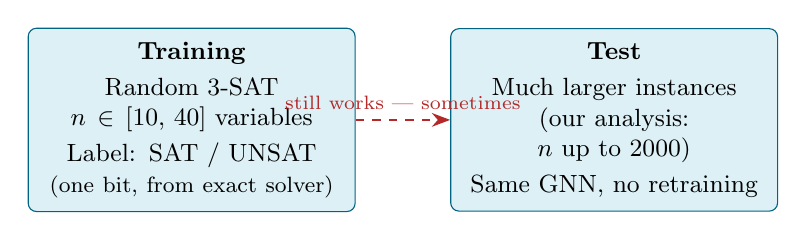
\begin{tikzpicture}[every node/.style={font=\small}]
  \node[box, text width=3.8cm] (tr) {
    \textbf{Training}\\[2pt]
    Random 3-SAT\\
    $n \in [10,\,40]$ variables\\[2pt]
    Label: SAT / UNSAT\\
    {\footnotesize (one bit, from exact solver)}
  };
  \node[box, text width=3.8cm, right=1.2cm of tr] (te) {
    \textbf{Test}\\[2pt]
    Much larger instances\\
    (our analysis: $n$ up to 2000)\\[2pt]
    Same GNN, no retraining
  };
  \draw[arrow, dashed, color=emphcolor] (tr.east) -- (te.west)
        node[midway, above, font=\scriptsize, color=emphcolor]
        {still works — sometimes};
\end{tikzpicture}

\column{0.44\textwidth}
\vspace{0.3cm}
\begin{block}{The puzzle}
\small
\textbf{Observation:} surprisingly strong generalization beyond training range.\\[4pt]
\textbf{Caveat:} we do not fully understand why this generalization happens.\\[4pt]
\textbf{Question:} what does the model encode internally?
\end{block}
\end{columns}
\note{I want to be precise. NeuroSAT did not solve SAT in an algorithmic sense —
its authors did not claim that. What it did, surprisingly, is generalize to much larger instances
than it was trained on with only a binary label. That train-small/test-large behavior created a
serious interpretability puzzle. We don't fully understand it yet. What we did is start asking: what
is encoded in the model's internal representations? That question, it turns out, has an answer.}
\end{frame}

% ── Slide 3 ──────────────────────────────────────────────────────────────────
\begin{frame}{The running question}
\begin{block}{Running question}
\large\centering
When a GNN appears to solve a hard combinatorial problem —\\
\textbf{what did it actually learn?}
\end{block}

\bigskip
\begin{tabular}{@{}lll@{}}
\toprule
\textbf{Chapter} & \textbf{Setting} & \textbf{Answer} \\
\midrule
1 & GNNs in general & \textit{[to be revealed]} \\
2 & SAT and Coloring & \textit{[to be revealed]} \\
3 & Max-Clique / Sparse PCA & \textit{[to be revealed]} \\
4 & SDP / OptGNN & \textit{[to be revealed]} \\
\bottomrule
\end{tabular}

\bigskip
\small\color{bgucolor}
I will return to this table at the end of each chapter.
\note{I'll return to this slide at the end of each chapter with the answer for that
setting. Think of it as a running scoreboard. The final slide closes the loop.}
\end{frame}

% ── Slide 4 ──────────────────────────────────────────────────────────────────
\begin{frame}{The setting: combinatorial optimization on graphs}
\begin{columns}[T]
\column{0.45\textwidth}
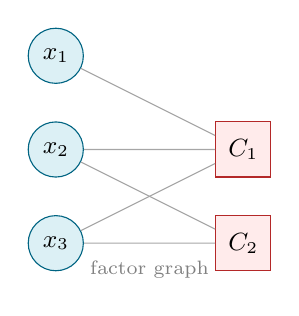
\begin{tikzpicture}[scale=0.85, every node/.style={font=\small}]
  % variable nodes
  \foreach \i/\lbl in {1/$x_1$, 2/$x_2$, 3/$x_3$} {
    \node[node] (v\i) at (0, -1.4*\i+2.1) {\lbl};
  }
  % clause nodes
  \foreach \j/\lbl in {1/$C_1$, 2/$C_2$} {
    \node[clause] (c\j) at (2.8, -1.4*\j+0.7) {\lbl};
  }
  % edges
  \draw[gray!70] (v1) -- (c1);
  \draw[gray!70] (v2) -- (c1);
  \draw[gray!70] (v2) -- (c2);
  \draw[gray!70] (v3) -- (c1);
  \draw[gray!70] (v3) -- (c2);
  \node[font=\scriptsize, color=gray] at (1.4, -2.5) {factor graph};
\end{tikzpicture}

\column{0.52\textwidth}
\begin{itemize}
  \item \textbf{Input:} graph or formula
  \item \textbf{Goal:} assignment satisfying all (or most) constraints
  \item \textbf{Hard:} NP-complete in the worst case
\end{itemize}
\medskip
\textbf{Problems in this talk:}
\begin{itemize}
  \item 3-\textbf{SAT}: assign TRUE/FALSE to variables
  \item \textbf{Coloring}: assign colors, no two adjacent vertices same
  \item \textbf{Clique}: find a large complete subgraph
  \item \textbf{Sparse PCA}: recover a sparse signal from a covariance matrix
\end{itemize}
\end{columns}
\note{These are canonical NP-hard problems. Each serves as a test case. Their
different structures will matter: when we ask what concept the GNN learned, the answer
depends on what structure the problem has.}
\end{frame}

% ── Slide 5 ──────────────────────────────────────────────────────────────────
\begin{frame}{Supervised learning in 60 seconds}
\begin{columns}[T]
\column{0.5\textwidth}
\textbf{General setup:}
\begin{itemize}
  \item Training data: \textit{(instance, label)} pairs
  \item Model: $f_\theta$: instance $\to$ prediction
  \item Loss: how wrong is $f_\theta$ vs.\ the label?
  \item Training: adjust $\theta$ to reduce loss
\end{itemize}

\bigskip
\textbf{For NeuroSAT:}
\begin{itemize}
  \item Instance: a SAT formula
  \item Label: \texttt{SAT} or \texttt{UNSAT} (one bit)
  \item Loss: cross-entropy on that single bit
\end{itemize}

\column{0.46\textwidth}
\begin{block}{Key point}
\small
The loss says \emph{nothing} about which variables should be TRUE, or about support,
degree, or any other solver concept.

\medskip
Those concepts are \textbf{not prescribed.}

\medskip
If they appear in the learned embeddings — they \textbf{emerged spontaneously.}
\end{block}
\end{columns}
\note{This is the key point about NeuroSAT's loss: it tells the model nothing
about how to solve SAT. It only says whether the formula is satisfiable. Everything the model
does internally is not required by the loss. That's the puzzle.}
\end{frame}

% ── Slide 6 ──────────────────────────────────────────────────────────────────
\begin{frame}{Train, test, and the generalization puzzle}

\begin{center}
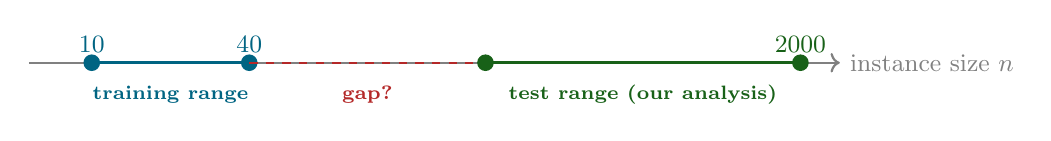
\begin{tikzpicture}[every node/.style={font=\small}]
  \draw[->, thick, gray] (-0.3,0) -- (10,0) node[right] {instance size $n$};
  % training range
  \draw[bgucolor, very thick] (0.5,0) -- (2.5,0);
  \fill[bgucolor] (0.5,0) circle(3pt) node[above] {$10$};
  \fill[bgucolor] (2.5,0) circle(3pt) node[above] {$40$};
  \node[bgucolor, font=\scriptsize] at (1.5, -0.4) {\textbf{training range}};
  % gap
  \draw[emphcolor, dashed, thick] (2.5,0) -- (5.5,0);
  \node[emphcolor, font=\scriptsize] at (4,-0.4) {\textbf{gap?}};
  % test range
  \draw[ForestGreen!70!black, very thick] (5.5,0) -- (9.5,0);
  \fill[ForestGreen!70!black] (5.5,0) circle(3pt) node[above] {};
  \fill[ForestGreen!70!black] (9.5,0) circle(3pt) node[above] {$2000$};
  \node[ForestGreen!70!black, font=\scriptsize] at (7.5,-0.4) {\textbf{test range (our analysis)}};
\end{tikzpicture}
\end{center}

\medskip
\begin{columns}[T]
\column{0.48\textwidth}
\textbf{Ordinary generalization:}\\same distribution, held-out examples
\column{0.48\textwidth}
\textbf{Size generalization:}\\test instances much larger than training
\end{columns}

\bigskip
\begin{alertblock}{}
\small
If the model generalizes across sizes:\\
$\Rightarrow$ it learned something \textbf{structural} — not instance-specific\\
$\Rightarrow$ that structural invariant is our object of study
\end{alertblock}
\note{When a model generalizes to instances from the same distribution and same
size, that's ordinary generalization. What's unusual here is cross-size generalization. It suggests
the model found an invariant of the problem structure that holds at all scales. That's what we're
hunting.}
\end{frame}

% ── Slide 7 ──────────────────────────────────────────────────────────────────
\begin{frame}{Four things to keep separate}
\small
\renewcommand{\arraystretch}{1.35}
\begin{tabular}{@{}p{3.2cm}p{5.5cm}p{2.5cm}@{}}
\toprule
\textbf{Component} & \textbf{What it is} & \textbf{Who decides} \\
\midrule
\textbf{Architecture} & how information flows (layers, message-passing graph) & researcher \\
\textbf{Parameters} $\theta$ & numerical values inside the model & \alert{learned from data} \\
\textbf{Training objective} & what the model is rewarded for predicting & researcher \\
\textbf{Decoding strategy} & how output scores $\to$ discrete solution & researcher (can be changed post-training) \\
\bottomrule
\end{tabular}

\bigskip
\begin{block}{When we say "the model learned $X$"}
\small
$X$ lives in the \textbf{parameters} — not designed, not prescribed by the loss.\\
$X$ emerged from the interaction of architecture, objective, and data.
\end{block}
\note{This distinction will matter a lot. When I say 'the GNN learned support,'
I mean support is decodable from the learned parameters — from the embeddings — even
though the loss never mentioned it. The concept emerged. That's the interesting part.}
\end{frame}

% ── Slide 8 ──────────────────────────────────────────────────────────────────
\begin{frame}{Graph-structured problems need graph-structured models}
\begin{columns}[T]
\column{0.5\textwidth}
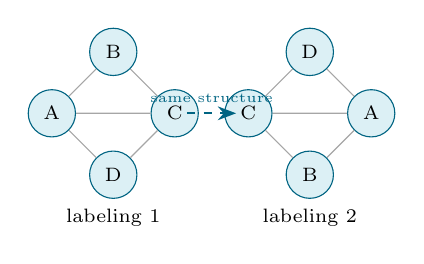
\begin{tikzpicture}[scale=0.78, every node/.style={font=\scriptsize}]
  % left graph
  \foreach \i/\x/\y in {A/0/1, B/1/2, C/2/1, D/1/0} {
    \node[circle, draw=bgucolor, fill=bgulight, minimum size=6mm] (\i) at (\x,\y) {\i};
  }
  \draw[gray!70] (A)--(B)--(C)--(D)--(A)--(C);
  \node at (1,-0.7) {labeling 1};
  % right graph (relabeled)
  \begin{scope}[xshift=3.2cm]
  \foreach \i/\x/\y in {C/0/1, D/1/2, A/2/1, B/1/0} {
    \node[circle, draw=bgucolor, fill=bgulight, minimum size=6mm] (\i r) at (\x,\y) {\i};
  }
  \draw[gray!70] (Cr)--(Dr)--(Ar)--(Br)--(Cr)--(Ar);
  \node at (1,-0.7) {labeling 2};
  \end{scope}
  \draw[arrow, dashed] (2.2,1) -- (3.0,1) node[midway, above, font=\tiny]{same structure};
\end{tikzpicture}

\column{0.46\textwidth}
\textbf{Challenge:}\\
same graph, different node labels $\to$ same structure

\medskip
Standard NN: \alert{fails} (no permutation invariance)\\
GNN: \textcolor{ForestGreen!70!black}{\textbf{operates on structure}} $\checkmark$

\medskip\textbf{Also:}
\begin{itemize}\small
  \item Variable-size graphs $\to$ GNNs handle naturally
  \item Constraints are local $\to$ local message passing fits
  \item Sparse graphs $\to$ GNNs scale with edges, not $n^2$
\end{itemize}
\end{columns}
\note{Combinatorial problems on graphs are permutation-invariant. GNNs are built
for this. They also scale linearly with the number of edges, making them usable on large sparse
instances.}
\end{frame}

% ── Slide 9 ──────────────────────────────────────────────────────────────────
\begin{frame}{What is a GNN?}
\begin{columns}[T]
\column{0.48\textwidth}
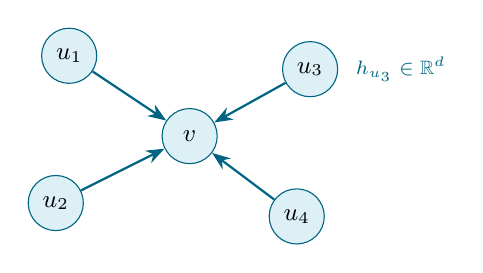
\begin{tikzpicture}[scale=0.85, every node/.style={font=\small}]
  \node[node] (v) at (2,2) {$v$};
  \node[node] (u1) at (0.2,3.2) {$u_1$};
  \node[node] (u2) at (0,1.0) {$u_2$};
  \node[node] (u3) at (3.8,3.0) {$u_3$};
  \node[node] (u4) at (3.6,0.8) {$u_4$};
  \draw[arrow] (u1) -- (v);
  \draw[arrow] (u2) -- (v);
  \draw[arrow] (u3) -- (v);
  \draw[arrow] (u4) -- (v);
  \node[font=\scriptsize, bgucolor, right=0.1cm of u3] {$h_{u_3}\in\mathbb{R}^d$};
\end{tikzpicture}

\column{0.48\textwidth}
Each vertex $v$ has a state $h_v \in \mathbb{R}^d$

\medskip
\textbf{Each round $t$:}
\[
  m_v \;=\; \mathrm{AGG}\!\bigl(\{h_u : u\in\mathcal{N}(v)\}\bigr)
\]
\[
  h_v \;\leftarrow\; \mathrm{UPDATE}(h_v,\, m_v)
\]

\medskip
After $T$ rounds: \textbf{predict} from $\{h_v\}$

\medskip\small
\texttt{AGG} and \texttt{UPDATE} are \textbf{learned} (MLP/GRU).\\
After $T$ rounds: $v$ has seen its $T$-hop neighborhood.
\end{columns}
\note{Think of it as a distributed algorithm where each node keeps a memory
vector and exchanges messages with its neighbors. The only difference from a designed algorithm
is that AGG and UPDATE are learned. What they learn to compute — that's our question.}
\end{frame}

% ── Slide 10 ─────────────────────────────────────────────────────────────────
\begin{frame}{Message passing in action}

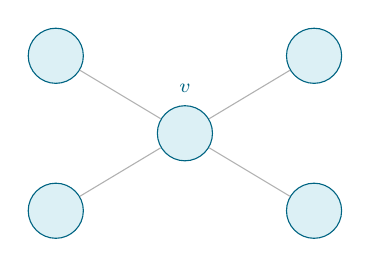
\begin{tikzpicture}[scale=0.82, every node/.style={font=\scriptsize}]
  % nodes
  \foreach \i/\x/\y in {v/3/1.8, u1/1/3, u2/1/0.6, u3/5/3, u4/5/0.6} {
    \node[node] (\i) at (\x, \y) {};
  }
  \node[above=1pt of v, font=\scriptsize, bgucolor] {$v$};
  \foreach \nd in {u1,u2,u3,u4} {
    \draw[gray!60] (\nd) -- (v);
  }
\end{tikzpicture}
\hfill
\begin{minipage}[t]{0.62\textwidth}
\small
\begin{overprint}
\onslide<1>
\textbf{Round 0:}
\begin{itemize}
  \item $h_v = \text{random}$ for all $v$
  \item All vertices look identical
\end{itemize}

\onslide<2>
\textbf{Round 1:}
\begin{itemize}
  \item $h_v \leftarrow \mathrm{UPDATE}(h_v,\, \mathrm{AGG}(\text{neighbors}))$
  \item $v$ now "knows about" its 1-hop neighborhood
\end{itemize}

\onslide<3>
\textbf{Round $T$:}
\begin{itemize}
  \item $v$ knows about its $T$-hop ball
  \item Embeddings encode local graph structure
\end{itemize}

\onslide<4>
\textbf{Readout:}
\[
  s_v = \mathrm{MLP}(h_v) \in [0,1]
\]
\textbf{Decoding:} top-$k$, LPR, or rounding\\
\alert{Designer's choice — not learned.}\\
(This matters in Chapter 3.)
\end{overprint}
\end{minipage}

\note{I'll use animations here. The key takeaway: after T rounds, each node has a
summary of its T-hop neighborhood. The scores come from the learned parameters. The decoder
is separate — and that distinction matters in Chapter 3.}
\end{frame}

% ── Slide 11 ─────────────────────────────────────────────────────────────────
\begin{frame}{Belief propagation: the classical template}

\begin{center}
\renewcommand{\arraystretch}{1.4}
\begin{tabular}{@{}p{3.5cm}p{3.8cm}p{3.8cm}@{}}
\toprule
 & \textbf{Classical BP} & \textbf{GNN} \\
\midrule
\textbf{Message} & scalar / probability & vector $\in \mathbb{R}^d$ \\
\textbf{Update rule} & analytically derived & learned (MLP/GRU) \\
\textbf{Objective} & probabilistic model & task loss (SAT/UNSAT) \\
\textbf{Convergence} & proven on trees & empirical \\
\textbf{Interpretability} & high & \alert{our question} \\
\bottomrule
\end{tabular}
\end{center}

\bigskip
\begin{block}{}
A GNN is \textbf{BP-inspired high-dimensional learned message passing.}\\
Not BP — but BP is the right mental model for this audience.
\end{block}

\note{BP passes structured probabilistic summaries; the GNN passes high-dimensional
learned vectors. BP derives its update analytically; the GNN learns it from data. The question of
what the GNN learned is, in a sense, a question about what it reinvented from the BP world. But
there's an important caveat — next slide.}
\end{frame}

% ── Slide 12 ─────────────────────────────────────────────────────────────────
\begin{frame}{The limits of the BP analogy}

\begin{center}
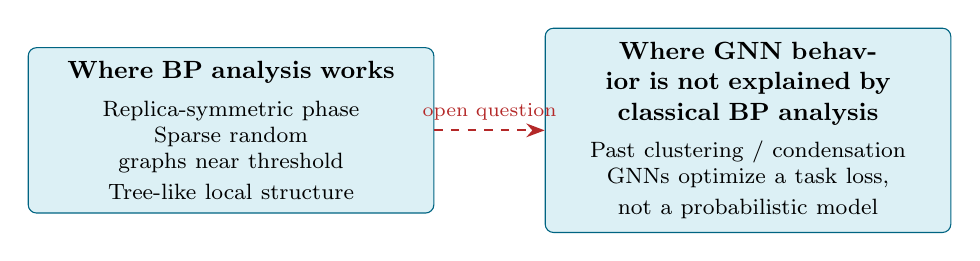
\begin{tikzpicture}[every node/.style={font=\small}]
  \node[box, text width=4.8cm] (left) {
    \textbf{Where BP analysis works}\\[4pt]
    \footnotesize
    Replica-symmetric phase\\
    Sparse random graphs near threshold\\
    Tree-like local structure
  };
  \node[box, text width=4.8cm, right=1.4cm of left] (right) {
    \textbf{Where GNN behavior is not explained by classical BP analysis}\\[4pt]
    \footnotesize
    Past clustering / condensation\\
    GNNs optimize a task loss,\\
    not a probabilistic model
  };
  \draw[arrow, dashed, emphcolor] (left.east) -- (right.west)
    node[midway, above, font=\scriptsize, emphcolor]{open question};
\end{tikzpicture}
\end{center}

\medskip\small
\begin{itemize}
  \item Classical BP has known failure regimes in random CSPs
  \item GNNs trained on task loss are not bound by those regimes in the same way
  \item Why GNNs sometimes work where BP analysis does not predict success is \textbf{part of the open puzzle}
  \item The concept-learning framework is \textit{one lens} into this — not the final answer
\end{itemize}

\note{Say this once and move on. BP is the analogy, not the claim. Classical BP
has known failure regimes; the point is that GNNs are learned high-dimensional message passing,
and part of the puzzle is why they sometimes behave better than this analogy predicts. We don't
fully understand this yet. Now, the result that started the puzzle.}
\end{frame}

% ── Slide 13 ─────────────────────────────────────────────────────────────────
\begin{frame}{NeuroSAT: the promise}
\begin{columns}[T]
\column{0.5\textwidth}
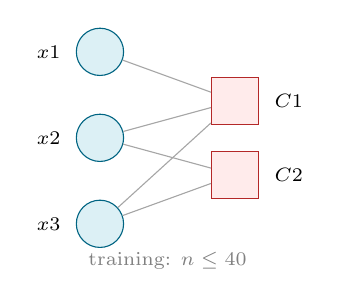
\begin{tikzpicture}[scale=0.78, every node/.style={font=\scriptsize}]
  % small factor graph
  \foreach \i/\x/\y in {x1/0/2.8, x2/0/1.4, x3/0/0} {
    \node[node, minimum size=6mm] (\i) at (\x,\y) {};
    \node[left=2pt of \i, font=\scriptsize] {$\i$};
  }
  \foreach \j/\y in {C1/2, C2/0.8} {
    \node[clause, minimum size=6mm] (\j) at (2.2,\y) {};
    \node[right=2pt of \j, font=\scriptsize] {$\j$};
  }
  \draw[gray!70] (x1)--(C1); \draw[gray!70] (x2)--(C1); \draw[gray!70] (x3)--(C1);
  \draw[gray!70] (x2)--(C2); \draw[gray!70] (x3)--(C2);
  \node[font=\scriptsize, color=gray] at (1.1,-0.6) {training: $n\le 40$};
\end{tikzpicture}

\column{0.46\textwidth}
\textbf{NeuroSAT} (Selsam et al., 2019):
\begin{itemize}\small
  \item Architecture: message-passing GNN on CNF factor graph
  \item Training: SAT/UNSAT label only — single-bit supervision
  \item Training set: $n \in [10, 40]$, near phase transition
\end{itemize}

\medskip
\textbf{Observation:}\\
\small Surprisingly strong generalization beyond training range\\
(our analysis: $n$ up to 2000)

\medskip
\textbf{Our question:}\\
\small What did it learn internally?
\end{columns}

\note{NeuroSAT is not a general SAT solver. What it showed is that a very simple
GNN, trained with one bit of supervision per instance, organized its internal representations
in a way that worked on much larger instances. That suggests it found something structural. Our
project is to name that something.}
\end{frame}

% ── Slide 14 ─────────────────────────────────────────────────────────────────
\begin{frame}{Chapter 1: partial answer + the research program}

\begin{block}{Running question — Chapter 1 answer (partial)}
\small
Possibly: a \textbf{transferable message-passing rule} capturing structural invariants.\\
But the training loss doesn't specify which rule. That is the interpretability puzzle.
\end{block}

\medskip
\textbf{Our method — concept learning:}
\begin{enumerate}\small
  \item Project learned embeddings to low-dimensional PCA space
  \item Ask: does the projection align with known algorithmic quantities?
  \item Verify: a simple linear probe predicts the concept on held-out instances
\end{enumerate}

\medskip
\textbf{A concept $g_\phi(v)$ is \textit{learned} iff:}
\[
  \hat{g}(v) = w^\top h_v + b \quad\text{predicts } g_\phi(v) \text{ on held-out instances}
\]
\small Falsifiable: fails if the quantity isn't predictable above baseline.

\note{The concept-learning framework is the methodological core. We don't assume
the model learned any particular thing. We ask whether classical algorithmic quantities are
encoded in the embeddings, and test that with a linear probe. If support is encoded, the probe
can predict it on instances the probe never saw. Let's see what we find.}
\end{frame}

% ══════════════════════════════════════════════════════════════════════════════
%  CHAPTER 2 — SAT and Coloring: Support as Confidence
% ══════════════════════════════════════════════════════════════════════════════

\section{Chapter 2 — SAT and Coloring}

% ── Slide 15 ─────────────────────────────────────────────────────────────────
\begin{frame}{Chapter 2: SAT and Coloring}

\begin{block}{Running question}
When a GNN appears to solve a hard combinatorial problem — what did it actually learn?
\end{block}

\bigskip
\begin{columns}[T]
\column{0.48\textwidth}
\textbf{Problem 1 — SAT}\\
\small Shoham, Cohen, Wattad, Rika, Vilenchik\\
\textit{Information Sciences} 726 (2026)

\medskip
GNN: NeuroSAT\\
Trained with single-bit binary supervision only.

\column{0.48\textwidth}
\textbf{Problem 2 — 3-Coloring}\\
\small Shoham, Rika, Vilenchik\\
AAAI 2025

\medskip
GNN: GNN-GCP\\
Trained with single-bit binary supervision only.
\end{columns}

\bigskip
\small\color{bgucolor} We probe their learned embeddings. Neither loss mentions any solver quantity.

\note{We now ask the running question for two constraint-satisfaction problems.
Both GNNs were trained with only a binary label. Neither loss mentions any solver quantity.
Here is what we found.}
\end{frame}

% ── Slide 16 ─────────────────────────────────────────────────────────────────
\begin{frame}{Concept learning for algorithmic tasks}

\begin{columns}[T]
\column{0.44\textwidth}
\textbf{Standard XAI:} which input features drove this decision?\\
\small (SHAP, LIME, GradCAM)

\medskip\small
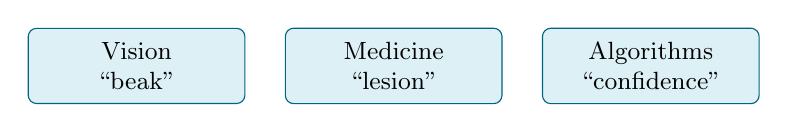
\begin{tikzpicture}
  \node[box, text width=2.4cm] (v) {Vision\\``beak''};
  \node[box, text width=2.4cm, right=0.5cm of v] (m) {Medicine\\``lesion''};
  \node[box, text width=2.4cm, right=0.5cm of m] (a) {\alert{Algorithms}\\``confidence''};
\end{tikzpicture}

\column{0.52\textwidth}
\textbf{For algorithmic tasks: features are not enough.}
\begin{itemize}\small
  \item ``$x_1$ appears in clause 7'' → instance-specific, not transferable
  \item ``$x_1$ has high support'' → \textbf{meaningful across instances}
\end{itemize}

\medskip
\begin{block}{A concept}
\small A compact quantity that \textbf{generalizes across instances,}\\
explains internal dynamics, and has algorithmic meaning.
\end{block}
\end{columns}

\note{We need concepts — not feature attributions for one input, but global
algorithmic quantities that explain how the model behaves across all instances. That requires
looking at the geometry of the internal representations over many runs.}
\end{frame}

% ── Slide 17 ─────────────────────────────────────────────────────────────────
\begin{frame}{SAT as a factor graph: the running example}

\begin{columns}[T]
\column{0.48\textwidth}
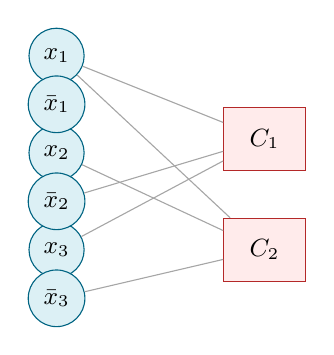
\begin{tikzpicture}[scale=0.88, every node/.style={font=\small}]
  % variable (literal) nodes
  \foreach \i/\lbl/\y in {1/$x_1$/4.2, 2/$x_2$/2.8, 3/$x_3$/1.4,
                           4/$\bar x_1$/3.5, 5/$\bar x_2$/2.1, 6/$\bar x_3$/0.7} {
    \node[node, minimum size=7mm] (lit\i) at (0, \y) {\lbl};
  }
  % clause nodes
  \node[clause, minimum size=8mm, text width=8mm, align=center] (C1) at (3, 3.0) {$C_1$};
  \node[clause, minimum size=8mm, text width=8mm, align=center] (C2) at (3, 1.4) {$C_2$};
  % C1 = (x1 v ~x2 v x3)
  \draw[gray!70] (lit1)--(C1); \draw[gray!70] (lit5)--(C1); \draw[gray!70] (lit3)--(C1);
  % C2 = (x1 v x2 v ~x3)
  \draw[gray!70] (lit1)--(C2); \draw[gray!70] (lit2)--(C2); \draw[gray!70] (lit6)--(C2);
\end{tikzpicture}

\column{0.48\textwidth}
\textbf{CNF formula:}\\
$(x_1 \vee \bar x_2 \vee x_3)\;\wedge\;(x_1 \vee x_2 \vee \bar x_3)$

\medskip
\textbf{Factor graph:}
\begin{itemize}\small
  \item \textcolor{bgucolor}{Variable nodes:} $x_1, x_2, x_3$ and negations
  \item \textcolor{emphcolor}{Clause nodes:} $C_1, C_2$
  \item \textbf{Edges:} literal $\leftrightarrow$ clause where literal appears
\end{itemize}

\medskip
\small NeuroSAT runs $T$ rounds of message passing on this graph.\\
We ask: what do embeddings encode after training?
\end{columns}

\note{NeuroSAT operates on the factor graph, not the formula directly. Literals and
clauses are both node types — just like in survey propagation. Now I'll tell you what we found
inside those node embeddings.}
\end{frame}

% ── Slide 18 ─────────────────────────────────────────────────────────────────
\begin{frame}{What is ``support''?}

\begin{columns}[T]
\column{0.5\textwidth}
\textbf{Definition.} Assignment $\phi$, variable $x$, clause $C$.

\medskip
$x$ \textbf{supports} $C$ under $\phi \;\iff$\\
\quad$C$ is satisfied, and $x$ is the \textbf{only} satisfied literal.\\
\quad (clause type \texttt{TFF}: True, False, False)

\medskip
\[
  \mathrm{support}_\phi(x) = \bigl|\{C : x \text{ alone satisfies } C\}\bigr|
\]

\medskip
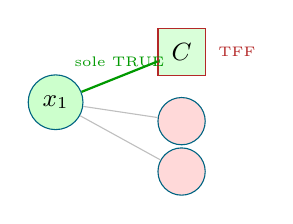
\begin{tikzpicture}[scale=0.8, every node/.style={font=\scriptsize}]
  \node[node, fill=green!20, minimum size=6mm] (x) at (0,0) {$x_1$};
  \node[clause, fill=green!15, minimum size=6mm] (c1) at (2,0.8) {$C$};
  \node[node, fill=red!15, minimum size=6mm] (x2) at (2,-0.3) {};
  \node[node, fill=red!15, minimum size=6mm] (x3) at (2,-1.1) {};
  \draw[green!60!black, thick] (x)--(c1) node[midway,above,font=\tiny,green!60!black]{sole TRUE};
  \draw[gray!50] (x)--(x2); \draw[gray!50] (x)--(x3);
  \node[right=1pt of c1, font=\tiny, emphcolor] {TFF};
\end{tikzpicture}

\column{0.46\textwidth}
\begin{block}{}
\small
\textbf{High support:}\\
$x$ is load-bearing $\to$ flipping $x$ breaks many clauses immediately.

\medskip
\textbf{Low support:}\\
$x$ is replaceable $\to$ safe to flip in local search.
\end{block}

\medskip\small
\textbf{This signal appears independently in:}
\begin{itemize}
  \item WalkSAT (local search)
  \item Survey Propagation (message passing)
  \item Backbone analysis (combinatorial structure)
\end{itemize}
\medskip
\alert{Three traditions, same concept.}
\end{columns}

\note{Support is a classical notion. Three very different algorithmic traditions —
WalkSAT (local search), Survey Propagation (message passing), backbone analysis
(combinatorial structure) — independently discovered the same signal. A variable with high
support is one you cannot safely change. It's a confidence signal. NeuroSAT, trained only on
SAT/UNSAT labels and never told about support, encodes precisely this quantity. Let me show you.}
\end{frame}

% ── Slide 19 ─────────────────────────────────────────────────────────────────
\begin{frame}{Support as confidence: a toy example}

\begin{columns}[T]
\column{0.48\textwidth}
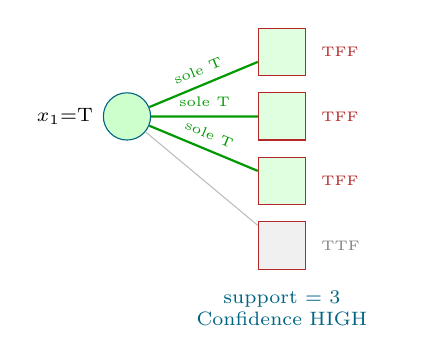
\begin{tikzpicture}[scale=0.82, every node/.style={font=\scriptsize}]
  \node[node, fill=green!20, minimum size=6mm, label=left:{$x_1$=T}] (x) at (0,2.4) {};
  % 3 TFF clauses
  \foreach \j/\y in {1/3.4, 2/2.4, 3/1.4} {
    \node[clause, fill=green!12, minimum size=6mm] (tc\j) at (2.4,\y) {};
    \draw[green!60!black, thick] (x) -- (tc\j)
      node[midway, above, sloped, font=\tiny, green!60!black]{sole T};
  }
  % 1 non-TFF
  \node[clause, fill=gray!12, minimum size=6mm] (tc4) at (2.4,0.4) {};
  \draw[gray!50] (x) -- (tc4);
  \node[right=2pt of tc1, font=\tiny, emphcolor] {TFF};
  \node[right=2pt of tc2, font=\tiny, emphcolor] {TFF};
  \node[right=2pt of tc3, font=\tiny, emphcolor] {TFF};
  \node[right=2pt of tc4, font=\tiny, gray] {TTF};
  \node[below=4pt of tc4, text width=3cm, align=center,
    font=\scriptsize, bgucolor]{support = 3\\Confidence HIGH};
\end{tikzpicture}

\column{0.48\textwidth}
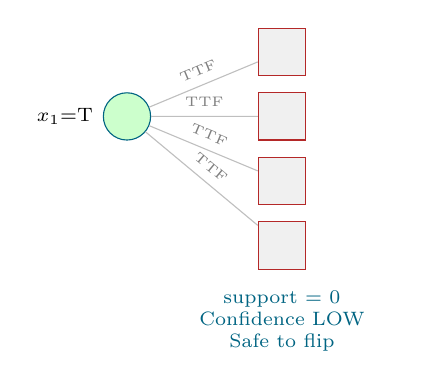
\begin{tikzpicture}[scale=0.82, every node/.style={font=\scriptsize}]
  \node[node, fill=green!20, minimum size=6mm, label=left:{$x_1$=T}] (x) at (0,2.4) {};
  \foreach \j/\y in {1/3.4, 2/2.4, 3/1.4, 4/0.4} {
    \node[clause, fill=gray!12, minimum size=6mm] (fc\j) at (2.4,\y) {};
    \draw[gray!50] (x) -- (fc\j) node[midway, above, sloped, font=\tiny, gray]{TTF};
  }
  \node[below=4pt of fc4, text width=3cm, align=center,
    font=\scriptsize, bgucolor]{support = 0\\Confidence LOW\\Safe to flip};
\end{tikzpicture}
\end{columns}

\note{If you were designing a local-search SAT solver, support is exactly the kind
of thing you'd track. NeuroSAT, which saw only binary SAT/UNSAT labels, encodes precisely
this. Let's look at the geometry.}
\end{frame}

% ── Slide 20 ─────────────────────────────────────────────────────────────────
\begin{frame}{NeuroSAT embeddings: PCA reveals support}

\begin{columns}[T]
\column{0.5\textwidth}
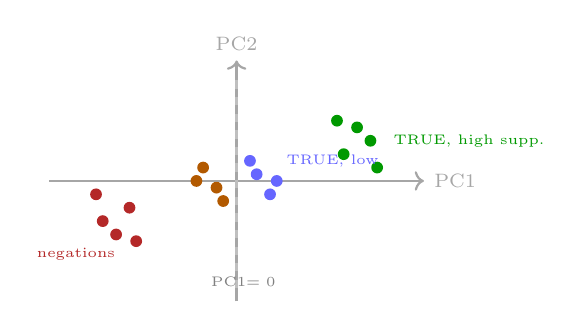
\begin{tikzpicture}[scale=0.85]
  % schematic PCA scatter plot
  \draw[->, thick, gray!70] (-2.8,0) -- (2.8,0) node[right, font=\scriptsize] {PC1};
  \draw[->, thick, gray!70] (0,-1.8) -- (0,1.8) node[above, font=\scriptsize] {PC2};
  % TRUE high-support (top-right)
  \foreach \x/\y in {1.6/0.4, 2.0/0.6, 1.8/0.8, 2.1/0.2, 1.5/0.9} {
    \fill[green!60!black] (\x,\y) circle(2.5pt);
  }
  % TRUE low-support (near center)
  \foreach \x/\y in {0.3/0.1, 0.5/-0.2, 0.2/0.3, 0.6/0.0} {
    \fill[blue!60] (\x,\y) circle(2.5pt);
  }
  % negations (mirror)
  \foreach \x/\y in {-1.6/-0.4, -2.0/-0.6, -1.8/-0.8, -2.1/-0.2, -1.5/-0.9} {
    \fill[emphcolor] (\x,\y) circle(2.5pt);
  }
  \foreach \x/\y in {-0.3/-0.1, -0.5/0.2, -0.2/-0.3, -0.6/0.0} {
    \fill[orange!70!black] (\x,\y) circle(2.5pt);
  }
  \node[font=\tiny, green!60!black, right] at (2.2,0.6) {TRUE, high supp.};
  \node[font=\tiny, blue!60, right] at (0.6,0.3) {TRUE, low};
  \node[font=\tiny, emphcolor] at (-2.4,-1.1) {negations};
  % symmetry arrow
  \draw[dashed, gray!50, thick] (0,-1.6) -- (0,1.6);
  \node[font=\tiny, gray] at (0.1,-1.5) {PC1$=0$};
\end{tikzpicture}

\column{0.46\textwidth}
\textbf{PCA of NeuroSAT's literal embeddings}\\
\small ($n = 1500$ variables, run to convergence)

\medskip
\begin{itemize}\small
  \item PC1 explains $\approx 90\%$ of variance
  \item PC2 explains $\approx 8\%$ of variance
  \item $\approx 98\%$ captured by 2 out of 128 dimensions
\end{itemize}

\medskip\small
PC1 value of a literal:\\
\quad\textbf{far positive} = TRUE, high support\\
\quad\textbf{near 0} = uncertain, low support\\
\quad\textbf{far negative} = negation

\medskip
\begin{block}{}
\small Linear probe: support is \textbf{predictable from embeddings} on held-out instances.
\end{block}
\end{columns}

\note{The model is 128-dimensional. 98% of what matters lives in 2 dimensions.
Those 2 dimensions encode support and assignment consistency. This is verified by a linear probe
on held-out instances — not just a visual impression.}
\end{frame}

% ── Slide 21 ─────────────────────────────────────────────────────────────────
\begin{frame}{Main finding: support governs NeuroSAT's dynamics}

\begin{columns}[T]
\column{0.5\textwidth}
\begin{block}{Theorem (informal)}
\small
Under assumptions on the distribution and simplified weights:\\
NeuroSAT's dynamics fix variables in \textbf{decreasing order of support,} starting with the $r$-support core — analogous to the graph-theoretic $r$-core.
\end{block}

\medskip\small
\textbf{Empirically:}
\begin{itemize}
  \item Variables with $|\mathrm{PC1}|$ near 0 are reassigned in the next iteration
  \item Variables far from 0 are locked in, consistent with a satisfying assignment
\end{itemize}

\column{0.46\textwidth}
\textbf{Payoffs from knowing this:}

\medskip
\textbf{StudentNeuroSAT:}\\
\small 91\% fewer parameters, comparable performance.

\medskip
\textbf{SupportSAT-01:}\\
\small WalkSAT variant guided by support signal. Faster convergence on $n = 1500$.

\medskip
\begin{alertblock}{}
\small
Concepts found by analysis\\$\to$ improved classical solvers.
\end{alertblock}
\end{columns}

\note{Two parts: a theoretical analysis showing the dynamics reduce to tracking
the support-core (for a simplified architecture), and the empirical probe. The concept is
immediately useful: it enables compression and algorithmic improvement.}
\end{frame}

% ── Slide 22 ─────────────────────────────────────────────────────────────────
\begin{frame}{Graph coloring: same concept, different geometry}

\begin{columns}[T]
\column{0.48\textwidth}
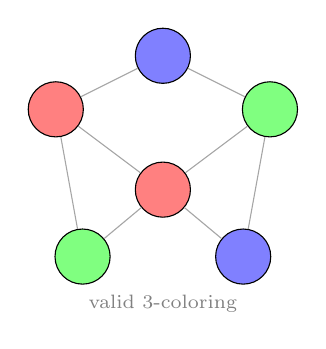
\begin{tikzpicture}[scale=0.85, every node/.style={font=\small}]
  % 3-colored graph
  \node[circle, draw, fill=red!50, minimum size=7mm] (v1) at (0,2.2) {};
  \node[circle, draw, fill=blue!50, minimum size=7mm] (v2) at (1.6,3.0) {};
  \node[circle, draw, fill=green!50, minimum size=7mm] (v3) at (3.2,2.2) {};
  \node[circle, draw, fill=red!50, minimum size=7mm] (v4) at (1.6,1.0) {};
  \node[circle, draw, fill=green!50, minimum size=7mm] (v5) at (0.4,0.0) {};
  \node[circle, draw, fill=blue!50, minimum size=7mm] (v6) at (2.8,0.0) {};
  \foreach \a/\b in {v1/v2, v2/v3, v3/v4, v4/v1, v1/v5, v3/v6, v5/v4, v6/v4} {
    \draw[gray!70] (\a)--(\b);
  }
  \node[font=\scriptsize, gray] at (1.6, -0.7) {valid 3-coloring};
\end{tikzpicture}

\column{0.48\textwidth}
\textbf{GNN-GCP} (Lemos et al., 2019):
\begin{itemize}\small
  \item Trained for 3-colorability (binary label only)
  \item Message-passing LSTM, 64-dim embeddings
\end{itemize}

\medskip
\textbf{Support in coloring:}\\
\small $\mathrm{support}(v)$ = number of neighbors in each color class other than its own

\medskip
\textbf{2D PCA projection:}
\begin{itemize}\small
  \item Embeddings form a \textbf{triangle}
  \item Color classes cluster near \textbf{corners}
  \item High-support vertices near corners (color-committed)
  \item Low-support near center (uncertain)
\end{itemize}
\end{columns}

\note{Support in coloring has an analogous meaning: the more neighbors of
conflicting colors, the more committed a vertex is to its own color. The GNN encodes this with
a triangular geometry. Color classes are the three corners of the triangle.}
\end{frame}

% ── Slide 23 ─────────────────────────────────────────────────────────────────
\begin{frame}{Support connects to a 1994 algorithm}

\begin{columns}[T]
\column{0.5\textwidth}
\small\renewcommand{\arraystretch}{1.3}
\begin{tabular}{@{}lp{4cm}@{}}
\toprule
& \textbf{Support meaning} \\
\midrule
\textbf{SAT} & clauses uniquely satisfied by $x$ \\
\textbf{Coloring} & neighbors $v$ has in each other color class \\
\midrule
\multicolumn{2}{l}{\small\textbf{In both:}} \\
\multicolumn{2}{l}{\small High support $\to$ high confidence $\to$ far from ambiguous region} \\
\multicolumn{2}{l}{\small Low support $\to$ uncertain $\to$ near center} \\
\bottomrule
\end{tabular}

\column{0.46\textwidth}
\textbf{This concept was hand-designed in:}
\begin{itemize}
  \item \textbf{WalkSAT} (1994) — for SAT
  \item \textbf{Alon–Kahale} (1994) — for graph coloring
\end{itemize}

\bigskip
\begin{alertblock}{}
\small
Across these two case studies, GNNs trained decades later \textbf{rediscover the same classical signal from data,} without supervision.
\end{alertblock}
\end{columns}

\note{The Alon-Kahale coloring algorithm from 1994 was designed around exactly
this support concept. The GNN, trained with no knowledge of that algorithm, encodes the same
quantity. Across these case studies, the GNNs don't appear to invent new primitives. They
appear to rediscover classical ones.}
\end{frame}

% ── Slide 24 ─────────────────────────────────────────────────────────────────
\begin{frame}{Chapter 2: running question answered}

\begin{block}{Running question — Chapter 2 answer (SAT and Coloring)}
\large\centering
\textbf{Support} — a classical confidence signal from solver theory.\\
\small Present in both GNNs, without supervision, across two different architectures.
\end{block}

\medskip
\small\renewcommand{\arraystretch}{1.25}
\begin{tabular}{@{}llp{4.2cm}@{}}
\toprule
\textbf{Problem} & \textbf{Concept} & \textbf{Evidence} \\
\midrule
SAT & Support & PCA + linear probe + theoretical analysis \textit{(formal + empirical)} \\
Coloring & Support (triangular) & Probe + embedding geometry \textit{(empirical / partly formal)} \\
\bottomrule
\end{tabular}

\medskip
\begin{alertblock}{}
\small
Does the same pattern hold for a structurally different problem?\\
$\to$ \textbf{Chapter 3: Max-Clique}
\end{alertblock}

\note{Chapter 2 answer: support. Two different GNNs, two different problems,
different architectures, different loss functions. Same emergent concept. Let's now move to a
structurally different problem — Max-Clique — and ask the same question.}
\end{frame}

% ══════════════════════════════════════════════════════════════════════════════
%  CHAPTER 3 — Clique: Degree, Ranking, and Cross-Domain Generalization
% ══════════════════════════════════════════════════════════════════════════════

\section{Chapter 3 — Max-Clique and Sparse PCA}

% ── Slide 25 ─────────────────────────────────────────────────────────────────
\begin{frame}{Chapter 3: Max-Clique}

\begin{block}{Running question}
When a GNN appears to solve a hard combinatorial problem — what did it actually learn?
\end{block}

\medskip
\begin{columns}[T]
\column{0.5\textwidth}
\textbf{Chapter 3 setting:}\\
\small Shoham, Haber, Rika, Vilenchik\\
AAAI 2026

\medskip
Problem: \textbf{Max-Clique}\\
No factor graph. No clause structure.\\
The signal lives in vertex degrees, not constraint satisfaction.

\column{0.46\textwidth}
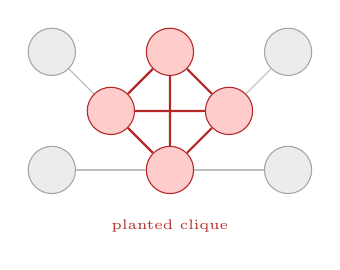
\begin{tikzpicture}[scale=0.75, every node/.style={font=\tiny}]
  % planted clique
  \foreach \i/\x/\y in {1/1/2, 2/2/3, 3/3/2, 4/2/1} {
    \node[circle, draw=emphcolor, fill=red!20, minimum size=6mm] (k\i) at (\x,\y) {};
  }
  \foreach \a/\b in {k1/k2, k1/k3, k1/k4, k2/k3, k2/k4, k3/k4} {
    \draw[emphcolor, thick] (\a)--(\b);
  }
  % background vertices
  \foreach \i/\x/\y in {5/0/3, 6/0/1, 7/4/3, 8/4/1} {
    \node[circle, draw=gray!70, fill=gray!15, minimum size=6mm] (bg\i) at (\x,\y) {};
  }
  \draw[gray!50] (bg5)--(k1); \draw[gray!50] (bg6)--(k4);
  \draw[gray!50] (bg7)--(k3); \draw[gray!50] (bg8)--(k4);
  \node[below=4pt, emphcolor] at (2,0.5) {planted clique};
\end{tikzpicture}
\end{columns}

\medskip\small\color{bgucolor}
If the concept-learning story is robust, it should survive this structural change.

\note{SAT and coloring have a natural factor-graph structure — that's where BP
is most natural. Clique is a different type of problem. The fact that a similar concept-learning
story holds there is a stronger test of the framework.}
\end{frame}

% ── Slide 26 ─────────────────────────────────────────────────────────────────
\begin{frame}{Planted clique: three difficulty regimes}

\begin{center}
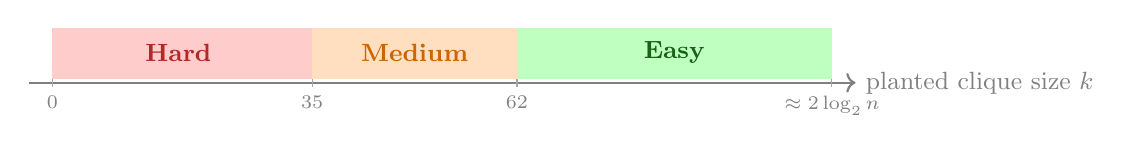
\begin{tikzpicture}[every node/.style={font=\small}]
  \draw[->, thick, gray] (0,0) -- (10.5,0) node[right, font=\small] {planted clique size $k$};
  % Easy
  \fill[green!25] (6.2,0.05) rectangle (10.2,0.7);
  \node[font=\small, ForestGreen!70!black] at (8.2, 0.38) {\textbf{Easy}};
  % Medium
  \fill[orange!25] (3.6,0.05) rectangle (6.2,0.7);
  \node[font=\small, orange!80!black] at (4.9, 0.38) {\textbf{Medium}};
  % Hard
  \fill[red!20] (0.3,0.05) rectangle (3.6,0.7);
  \node[font=\small, emphcolor] at (1.9, 0.38) {\textbf{Hard}};
  % tick marks
  \foreach \x/\lbl in {0.3/0, 3.6/35, 6.2/62, 10.2/{$\approx 2\log_2 n$}} {
    \draw[gray!70] (\x, -0.05) -- (\x, 0.05);
    \node[below, font=\scriptsize, gray] at (\x, -0.05) {\lbl};
  }
\end{tikzpicture}
\end{center}

\small\renewcommand{\arraystretch}{1.3}
\begin{tabular}{@{}p{1.6cm}p{3.5cm}p{4.5cm}@{}}
\toprule
\textbf{Regime} & \textbf{$k$ range ($n=1000$)} & \textbf{Known algorithms} \\
\midrule
Easy & $k \ge 62$ & Top-$k$ by degree recovers clique \\
Medium & $k \in [36, 61]$ & LPR or spectral methods needed \\
Hard & $k \le 35$ & Planted clique conjecture; no known efficient algorithm \\
\bottomrule
\end{tabular}

\note{We evaluate GNNs on instances calibrated to this landscape. Without
hardness control, you can't tell whether a GNN 'solving' clique is impressive or trivial.
Previous GNN evaluations for clique typically used uncontrolled benchmarks — that's part of the
methodological contribution here.}
\end{frame}

% ── Slide 27 ─────────────────────────────────────────────────────────────────
\begin{frame}{Degree as a classical signal: helpful but noisy}

\begin{columns}[T]
\column{0.5\textwidth}
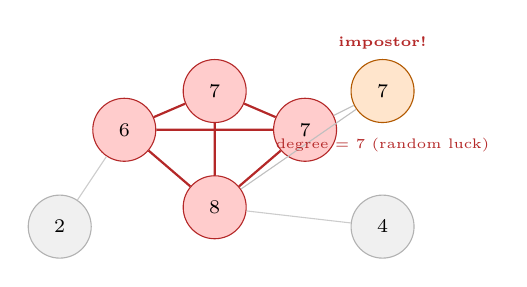
\begin{tikzpicture}[scale=0.82, every node/.style={font=\scriptsize}]
  % clique vertices
  \foreach \i/\x/\y/\deg in {1/1.0/3.0/6, 2/2.4/3.6/7, 3/3.8/3.0/7, 4/2.4/1.8/8} {
    \node[circle, draw=emphcolor, fill=red!20, minimum size=8mm] (k\i) at (\x,\y) {\deg};
  }
  \foreach \a/\b in {k1/k2, k1/k3, k1/k4, k2/k3, k2/k4, k3/k4} {
    \draw[emphcolor, thick] (\a)--(\b);
  }
  % impostor
  \node[circle, draw=orange!70!black, fill=orange!20, minimum size=8mm,
        label={[font=\tiny, emphcolor]above:\textbf{impostor!}}] (imp) at (5.0,3.6) {7};
  \draw[gray!50] (k3)--(imp);
  \draw[gray!50] (k4)--(imp);
  % non-clique
  \foreach \i/\x/\y/\deg in {5/0/1.5/2, 6/5/1.5/4} {
    \node[circle, draw=gray!60, fill=gray!12, minimum size=8mm] (nc\i) at (\x,\y) {\deg};
  }
  \draw[gray!40] (nc5)--(k1); \draw[gray!40] (nc6)--(k4);
  \node[font=\tiny, emphcolor, below=2pt of imp] {degree = 7 (random luck)};
\end{tikzpicture}

\column{0.46\textwidth}
\textbf{Degree heuristic:}
\begin{itemize}\small
  \item Clique vertices get degree ``boost'' from within-clique edges
  \item Sort by degree, take top $k$
\end{itemize}

\medskip
\textbf{Works in Easy regime.}\\
\textbf{Fails in Medium/Hard:}
\begin{itemize}\small
  \item ``Impostors'' — non-clique vertices with high random degree — enter top $k$
  \item The candidate set is not a valid clique
\end{itemize}

\medskip
\begin{block}{}
\small
What signal, beyond raw degree, distinguishes clique vertices in the Medium regime?
\end{block}
\end{columns}

\note{The degree heuristic is the simplest possible approach. In easy cases it's
enough. In medium and hard cases it's fooled by impostors. The question is whether the GNN
does something more clever — or whether it just learns a sophisticated version of degree.}
\end{frame}

% ── Slide 28 ─────────────────────────────────────────────────────────────────
\begin{frame}{What the GNN learns: degree-based ranking}

\begin{columns}[T]
\column{0.5\textwidth}
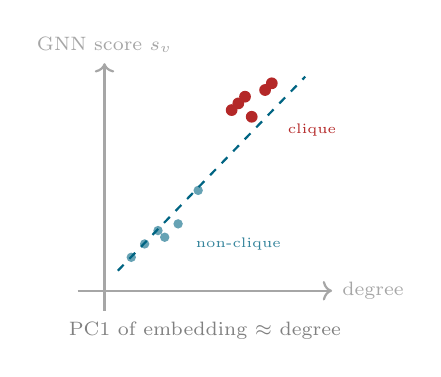
\begin{tikzpicture}[scale=0.85]
  \draw[->, gray!70, thick] (-0.4,0) -- (3.4,0) node[right, font=\scriptsize] {degree};
  \draw[->, gray!70, thick] (0,-0.3) -- (0,3.4) node[above, font=\scriptsize] {GNN score $s_v$};
  % scatter: clique vertices
  \foreach \x/\y in {2.0/2.8, 2.2/2.6, 2.4/3.0, 2.1/2.9, 2.5/3.1, 1.9/2.7} {
    \fill[emphcolor] (\x, \y) circle(2.5pt);
  }
  % scatter: non-clique
  \foreach \x/\y in {0.4/0.5, 0.8/0.9, 1.1/1.0, 0.6/0.7, 1.4/1.5, 0.9/0.8} {
    \fill[bgucolor!60] (\x, \y) circle(2pt);
  }
  % trend line
  \draw[bgucolor, dashed, thick] (0.2, 0.3) -- (3.0, 3.2);
  \node[font=\tiny, emphcolor] at (3.1, 2.4) {clique};
  \node[font=\tiny, bgucolor!80] at (2.0, 0.7) {non-clique};
  \node[font=\scriptsize, gray, align=center] at (1.5, -0.6) {PC1 of embedding $\approx$ degree};
\end{tikzpicture}

\column{0.46\textwidth}
\textbf{GNN embedding analysis (PCA):}
\begin{itemize}\small
  \item PC1 of vertex embeddings: highly correlated with vertex degree
  \item GNN output scores $\approx$ monotone function of degree
\end{itemize}

\medskip
\begin{block}{Finding (across these case studies)}
\small
The GNN learns \textbf{degree-based ranking.}\\
It does not appear to learn a fundamentally new signal.
\end{block}

\medskip\small
\textbf{But the decoder matters:}\\
Top-$k$ with degree fails on medium instances.\\
A smarter decoder changes the outcome substantially.
\end{columns}

\note{The GNN is doing sophisticated degree estimation — multi-hop, so better than
raw degree, but the principle is the same. The interesting result is what happens when you pair
this concept with the right decoder.}
\end{frame}

% ── Slide 29 ─────────────────────────────────────────────────────────────────
\begin{frame}{Top-$k$ vs.\ LPR: same concept, very different decoding}

\begin{columns}[T]
\column{0.48\textwidth}
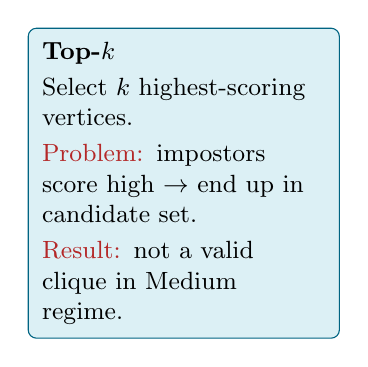
\begin{tikzpicture}[scale=0.78, every node/.style={font=\scriptsize}]
  \node[box, text width=3.6cm, align=left] (topk) {
    \textbf{Top-$k$}\\[2pt]
    Select $k$ highest-scoring vertices.\\[2pt]
    \textcolor{emphcolor}{Problem:} impostors score high $\to$ end up in candidate set.\\[2pt]
    \textcolor{emphcolor}{Result:} not a valid clique in Medium regime.
  };
\end{tikzpicture}

\column{0.48\textwidth}
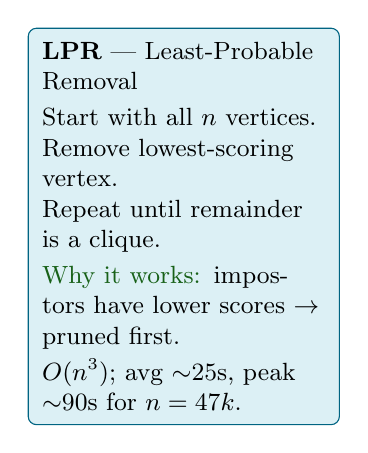
\begin{tikzpicture}[scale=0.78, every node/.style={font=\scriptsize}]
  \node[box, text width=3.6cm, align=left] (lpr) {
    \textbf{LPR} — Least-Probable Removal\\[2pt]
    Start with all $n$ vertices.\\
    Remove lowest-scoring vertex.\\
    Repeat until remainder is a clique.\\[2pt]
    \textcolor{ForestGreen!70!black}{Why it works:} impostors have lower scores $\to$ pruned first.\\[2pt]
    $O(n^3)$; avg $\sim$25s, peak $\sim$90s for $n=47k$.
  };
\end{tikzpicture}
\end{columns}

\bigskip
\begin{alertblock}{}
\small
LPR \textbf{significantly outperforms} Top-$k$ in Medium and Hard regimes.\\
Lesson: the concept (degree ranking) is in the scores; the decoding strategy determines how well you extract it.
\end{alertblock}

\note{LPR inverts the perspective: instead of selecting likely clique vertices, it
prunes unlikely ones. When impostors are present, they have lower scores — LPR removes them.
Same learned concept, very different decoding strategy, substantially different results.}
\end{frame}

% ── Slide 30 ─────────────────────────────────────────────────────────────────
\begin{frame}{Cross-domain transfer: the same GNN solves Sparse PCA}

\begin{columns}[T]
\column{0.5\textwidth}
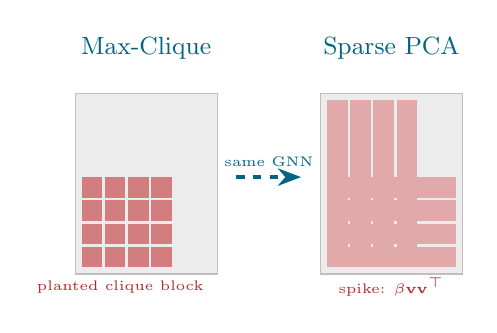
\begin{tikzpicture}[scale=0.82, every node/.style={font=\scriptsize}]
  % Planted clique matrix sketch
  \node[font=\small, bgucolor] at (1.1, 3.5) {Max-Clique};
  \fill[gray!15] (0,0) rectangle (2.2, 2.8);
  \foreach \i in {1,...,4} {
    \foreach \j in {1,...,4} {
      \fill[emphcolor!60] ({0.1+(\i-1)*0.36}, {0.1+(\j-1)*0.36}) rectangle
                          ({0.1+(\i-1)*0.36+0.32}, {0.1+(\j-1)*0.36+0.32});
    }
  }
  \draw[gray!50] (0,0) rectangle (2.2,2.8);
  \node[font=\tiny, emphcolor] at (0.7, -0.2) {planted clique block};
  % arrow
  \draw[arrow, dashed, very thick, bgucolor] (2.5,1.5) -- (3.5,1.5)
    node[midway, above, font=\tiny, bgucolor]{same GNN};
  % PCA matrix sketch
  \begin{scope}[xshift=3.8cm]
  \node[font=\small, bgucolor] at (1.1, 3.5) {Sparse PCA};
  \fill[gray!15] (0,0) rectangle (2.2, 2.8);
  \foreach \i in {1,...,4} {
    \fill[emphcolor!40] ({0.1+(\i-1)*0.36}, 0.1) rectangle
                        ({0.1+(\i-1)*0.36+0.32}, 2.7);
    \fill[emphcolor!40] (0.1, {0.1+(\i-1)*0.36}) rectangle
                        (2.1, {0.1+(\i-1)*0.36+0.32});
  }
  \draw[gray!50] (0,0) rectangle (2.2,2.8);
  \node[font=\tiny, emphcolor] at (1.1,-0.2) {spike: $\beta \mathbf{v}\mathbf{v}^\top$};
  \end{scope}
\end{tikzpicture}

\column{0.46\textwidth}
\textbf{Sparse PCA} (single-spike model):
\[
  \Sigma = I + \beta \mathbf{v}\mathbf{v}^\top, \quad \mathbf{v}\text{ sparse (size }k\text{)}
\]
Goal: recover support of $\mathbf{v}$.

\medskip
\textbf{Structural connection:}
\begin{itemize}\small
  \item Clique vertices: higher degree from within-clique edges
  \item Spike variables: larger row-sums from $\beta\mathbf{v}\mathbf{v}^\top$ perturbation
\end{itemize}

\medskip
\textbf{Transfer:}\\
\small GNN trained on Clique $\to$ Sparse PCA: succeeds.\\
GNN trained on Sparse PCA $\to$ Clique: succeeds.

\medskip
\begin{block}{}
\small
Learned principle: \textbf{row-sum ranking} — universal across both domains.\\
Matches Covariance Thresholding in the tested regime, without problem-specific hyperparameters.
\end{block}
\end{columns}

\note{We trained a GNN to find cliques. We gave it a covariance matrix from Sparse
PCA — a completely different problem. It succeeds because both problems have the same
underlying structure: identify a small subset with elevated row-sums. In learning degree ranking
for cliques, the GNN learned row-sum ranking in general. The exact claim is in the paper and backup slide B6.}
\end{frame}

% ── Slide 31 ─────────────────────────────────────────────────────────────────
\begin{frame}{Chapter 3: running question answered}

\begin{block}{Running question — Chapter 3 answer (Max-Clique / Sparse PCA)}
\large\centering
\textbf{Degree-based (row-sum) ranking} — a classical planted-graph signal.\\
\small Transfers across domains without retraining.
\end{block}

\medskip
\small\renewcommand{\arraystretch}{1.3}
\begin{tabular}{@{}llp{5cm}@{}}
\toprule
\textbf{Chapter} & \textbf{Problem} & \textbf{Emergent concept} \\
\midrule
2 & SAT / Coloring & Support (classical confidence signal) \\
3 & Clique / Sparse PCA & Degree-based row-sum ranking (classical planted-graph signal) \\
\bottomrule
\end{tabular}

\medskip
\begin{alertblock}{}
\small
\textbf{Theme (across these case studies):}\\
Different problem structures $\to$ different classical concepts.\\
But each concept was known. None appears to be a genuinely new primitive.
\end{alertblock}

\smallskip\small\color{bgucolor}
Chapter 4: What must a model learn in order to \textit{solve,} not just \textit{approximate}?

\note{Chapter 3 answer: degree ranking. Different from support, but again a
classical signal. In Chapter 4 we flip the question: instead of asking what a given model learned
post-hoc, we ask what concept is necessary for a model to cross the threshold from approximating
to solving.}
\end{frame}

% ══════════════════════════════════════════════════════════════════════════════
%  CHAPTER 4 — The Last Percent
% ══════════════════════════════════════════════════════════════════════════════

\section{Chapter 4 — The Last Percent}

% ── Slide 32 ─────────────────────────────────────────────────────────────────
\begin{frame}{Chapter 4: SDP / OptGNN}

\begin{block}{Running question — new angle}
Instead of asking what a given model learned,\\
we ask: \textbf{what must a model learn in order to \textit{solve,} not just \textit{approximate}?}
\end{block}

\bigskip
\textbf{Setting:}
\begin{itemize}
  \item OptGNN (Yau et al., NeurIPS 2024) and controlled variants
  \item Problems: SAT and NAE-SAT (hypergraph 2-coloring)
  \item Controlled design experiment: four architectural variants,\\
        progressively closer to explicit constraint structure
\end{itemize}

\medskip\small\color{bgucolor}
\textit{Note: results in this chapter are from a submitted manuscript. Exact numerical values are schematic.}

\note{This chapter turns the question around. Instead of reverse-engineering a
trained model, we run a controlled experiment. We start from a well-understood architecture,
make three principled modifications, and ask which one enables solving. The answer connects
back to everything in Chapters 2 and 3.}
\end{frame}

% ── Slide 33 ─────────────────────────────────────────────────────────────────
\begin{frame}{The approximation–solving gap}

\begin{center}
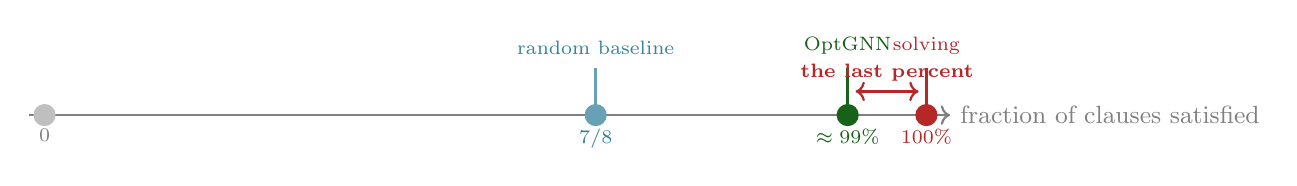
\begin{tikzpicture}[every node/.style={font=\small}]
  \draw[->, thick, gray] (-0.2,0) -- (11.5,0) node[right] {fraction of clauses satisfied};
  % baseline
  \fill[gray!50] (0,0) circle(4pt);
  \node[below, font=\scriptsize, gray] at (0,-0.05) {$0$};
  \draw[bgucolor!60, very thick] (7.0,0) -- (7.0,0.6);
  \fill[bgucolor!60] (7.0,0) circle(4pt);
  \node[below, font=\scriptsize, bgucolor!80] at (7.0,-0.05) {$7/8$};
  \node[above, font=\scriptsize, bgucolor!80] at (7.0, 0.65) {random baseline};
  % OptGNN
  \draw[ForestGreen!70!black, very thick] (10.2,0) -- (10.2, 0.6);
  \fill[ForestGreen!70!black] (10.2,0) circle(4pt);
  \node[below, font=\scriptsize, ForestGreen!70!black] at (10.2,-0.05) {$\approx 99\%$};
  \node[above, font=\scriptsize, ForestGreen!70!black] at (10.2, 0.65) {OptGNN};
  % Solving
  \draw[emphcolor, very thick] (11.2,0) -- (11.2, 0.6);
  \fill[emphcolor] (11.2,0) circle(4pt);
  \node[below, font=\scriptsize, emphcolor] at (11.2,-0.05) {$100\%$};
  \node[above, font=\scriptsize, emphcolor] at (11.2, 0.65) {solving};
  % gap label
  \draw[<->, emphcolor, thick] (10.3, 0.3) -- (11.1, 0.3)
    node[midway, above, font=\scriptsize, emphcolor]{\textbf{the last percent}};
\end{tikzpicture}
\end{center}

\small
\begin{itemize}
  \item \textbf{Random assignment:} satisfies each clause w.p.\ $7/8 = 87.5\%$ — trivially achievable
  \item \textbf{OptGNN} (Yau et al., NeurIPS 2024): reaches $\approx 99\%$
  \item \textbf{Worst-case hardness} (Håstad, 2001): even small improvements over $7/8$ are NP-hard in general — motivates taking the gap seriously
  \item \textbf{For random instances:} the last 1\% reflects a different barrier — coordinated changes across many variables simultaneously
  \item (Worst-case inapproximability $\neq$ random-instance hardness, but both are real.)
\end{itemize}

\begin{alertblock}{}
\small From $\approx 99\%$ to $100\%$ is a \textbf{qualitative transition,} not a marginal gain.
\end{alertblock}

\note{An assignment satisfying 99% of clauses can still be far from any satisfying
assignment — the last violated clauses may trigger cascades of required changes. The gap between
strong approximation and exact solving is the focus of this chapter.}
\end{frame}

% ── Slide 34 ─────────────────────────────────────────────────────────────────
\begin{frame}{OptGNN: SDP relaxations built into a GNN}

\begin{center}
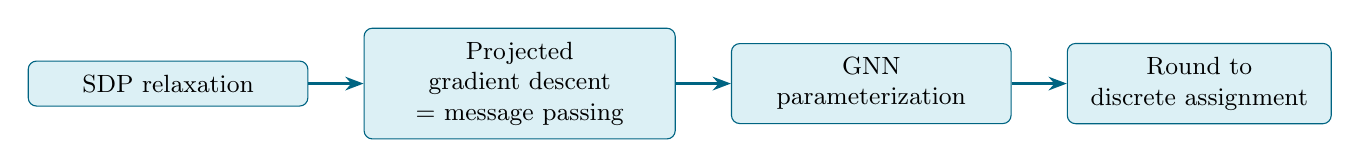
\begin{tikzpicture}[every node/.style={font=\small}]
  \node[box, text width=3.2cm] (sdp) {SDP relaxation};
  \node[box, text width=3.6cm, right=0.7cm of sdp] (gd) {Projected\\gradient descent\\= message passing};
  \node[box, text width=3.2cm, right=0.7cm of gd] (gnn) {GNN\\parameterization};
  \node[box, text width=3.0cm, right=0.7cm of gnn] (inf) {Round to\\discrete assignment};
  \draw[arrow] (sdp) -- (gd);
  \draw[arrow] (gd)  -- (gnn);
  \draw[arrow] (gnn) -- (inf);
\end{tikzpicture}
\end{center}

\medskip
\begin{columns}[T]
\column{0.5\textwidth}
\textbf{Key insight:} solving a certain SDP via projected gradient descent \textit{equals} message passing on the graph.\\
$\to$ architecture derived from an algorithm.

\medskip
\textbf{Training:} continuous SDP-inspired unsupervised loss.

\column{0.46\textwidth}
\textbf{Result:} near-optimal approximation on Max-Cut, Max-3-SAT, Min-Vertex-Cover (UGC-optimal guarantees)

\medskip
\textbf{Limitation:} strong approximation, but often fails to satisfy all constraints exactly.
\end{columns}

\note{OptGNN is an elegant construction — the architecture is derived from an
approximation algorithm. It has provable guarantees under the Unique Games Conjecture. But
its loss function is a continuous relaxation, not designed to enforce discrete feasibility. That's
the tension.}
\end{frame}

% ── Slide 35 ─────────────────────────────────────────────────────────────────
\begin{frame}{Three controlled modifications}

\begin{center}
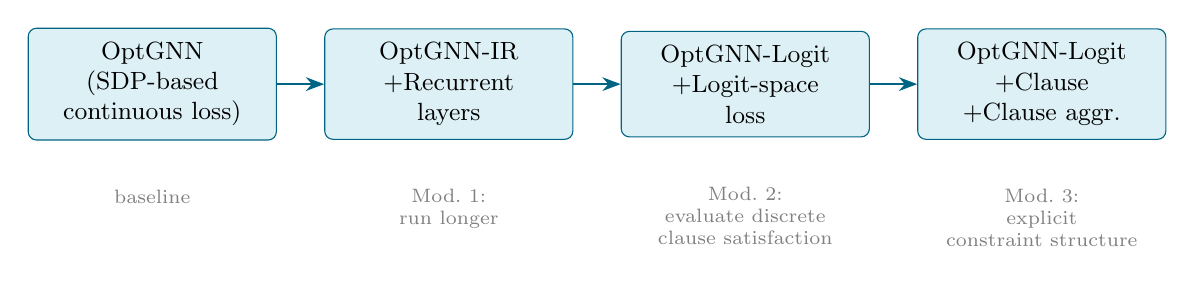
\begin{tikzpicture}[every node/.style={font=\small}]
  \node[box, text width=2.8cm] (v0) {OptGNN\\(SDP-based\\continuous loss)};
  \node[box, text width=2.8cm, right=0.6cm of v0] (v1) {OptGNN-IR\\+Recurrent\\layers};
  \node[box, text width=2.8cm, right=0.6cm of v1] (v2) {OptGNN-Logit\\+Logit-space\\loss};
  \node[box, text width=2.8cm, right=0.6cm of v2] (v3) {OptGNN-Logit\\+Clause\\+Clause aggr.};
  \draw[arrow] (v0)--(v1);
  \draw[arrow] (v1)--(v2);
  \draw[arrow] (v2)--(v3);
  \node[below=0.5cm of v0, font=\scriptsize, gray, text width=2.8cm, align=center] {baseline};
  \node[below=0.5cm of v1, font=\scriptsize, gray, text width=2.8cm, align=center]
    {Mod.~1:\\run longer};
  \node[below=0.5cm of v2, font=\scriptsize, gray, text width=2.8cm, align=center]
    {Mod.~2:\\evaluate discrete\\clause satisfaction};
  \node[below=0.5cm of v3, font=\scriptsize, gray, text width=2.8cm, align=center]
    {Mod.~3:\\explicit\\constraint structure};
\end{tikzpicture}
\end{center}

\small
\begin{itemize}
  \item \textbf{Mod.~1} (Recurrent layers): single recurrent unit, more iterations. Analogy: run a heuristic longer.
  \item \textbf{Mod.~2} (Logit-space loss): add rounding layer; loss evaluates discrete clause satisfaction directly.
  \item \textbf{Mod.~3} (Clause aggregation): explicit variable–constraint bipartite structure (factor-graph view built in).
\end{itemize}

\note{Each modification is inspired by classical heuristic design, not arbitrary
architecture search. Modification 1 is doing more of the same. Modifications 2 and 3 change
the qualitative structure of what information the model can form.}
\end{frame}

% ── Slide 36 ─────────────────────────────────────────────────────────────────
\begin{frame}{A sharp transition: approximation doesn't predict solving}

\begin{columns}[T]
\column{0.48\textwidth}
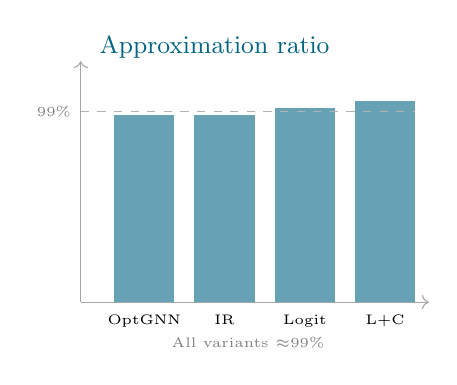
\begin{tikzpicture}[scale=0.85]
  % approximation bar chart
  \node[font=\small, bgucolor] at (2, 3.8) {Approximation ratio};
  \foreach \i/\lbl/\bh in {1/OptGNN/2.8, 2/IR/2.8, 3/Logit/2.9, 4/{L+C}/3.0} {
    \fill[bgucolor!60] ({0.5+(\i-1)*1.2}, 0) rectangle ({0.5+(\i-1)*1.2+0.9}, \bh);
    \node[below, font=\tiny] at ({0.95+(\i-1)*1.2}, -0.05) {\lbl};
  }
  \draw[->, gray!70] (0,0) -- (5.2,0);
  \draw[->, gray!70] (0,0) -- (0,3.6);
  \node[left, font=\tiny, gray] at (0, 2.85) {$99\%$};
  \draw[dashed, gray!60] (0, 2.85) -- (5.0, 2.85);
  \node[font=\tiny, gray, align=center] at (2.5, -0.6) {All variants $\approx$99\%};
\end{tikzpicture}

\column{0.48\textwidth}
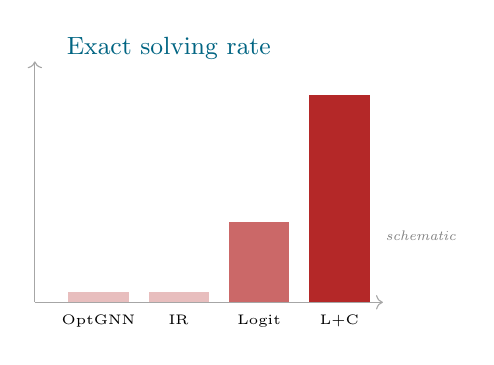
\begin{tikzpicture}[scale=0.85]
  % solving rate bar chart
  \node[font=\small, bgucolor] at (2, 3.8) {Exact solving rate};
  \fill[emphcolor!30] (0.5, 0) rectangle (1.4, 0.15);
  \fill[emphcolor!30] (1.7, 0) rectangle (2.6, 0.15);
  \fill[emphcolor!70] (2.9, 0) rectangle (3.8, 1.2);
  \fill[emphcolor] (4.1, 0) rectangle (5.0, 3.1);
  \foreach \i/\lbl in {1/OptGNN, 2/IR, 3/Logit, 4/{L+C}} {
    \node[below, font=\tiny] at ({0.95+(\i-1)*1.2}, -0.05) {\lbl};
  }
  \draw[->, gray!70] (0,0) -- (5.2,0);
  \draw[->, gray!70] (0,0) -- (0,3.6);
  \node[font=\tiny, color=gray, right] at (5.1, 1.0) {\textit{schematic}};
\end{tikzpicture}
\end{columns}

\medskip
\begin{alertblock}{}
\small
More iterations (Modification 1) alone \textbf{do not help.}\\
The transition requires a \textbf{qualitative architectural change.}\\
When it happens, it is \textbf{sharp} — not gradual.
\end{alertblock}

\note{You can run OptGNN longer — it still fails to solve. More iterations are not
enough. The transition requires changing what information the model can form. And when the
transition happens, it's discontinuous. Models go from near-zero solving to consistent solving.
There is no gradual middle ground.}
\end{frame}

% ── Slide 37 ─────────────────────────────────────────────────────────────────
\begin{frame}{Confidence bridges approximation and solving}

\begin{columns}[T]
\column{0.5\textwidth}
\small\renewcommand{\arraystretch}{1.4}
\begin{tabular}{@{}p{2.8cm}cc@{}}
\toprule
\textbf{Variant} & \textbf{Support decodable?} & \textbf{Solves?} \\
\midrule
OptGNN & \textcolor{emphcolor}{No} & \textcolor{emphcolor}{No} \\
OptGNN-IR & \textcolor{emphcolor}{No} & \textcolor{emphcolor}{No} \\
OptGNN-Logit & \textcolor{orange!80!black}{Partially} & \textcolor{orange!80!black}{Sometimes} \\
OptGNN-L+C & \textcolor{ForestGreen!70!black}{\textbf{Yes}} & \textcolor{ForestGreen!70!black}{\textbf{Yes}} \\
\bottomrule
\end{tabular}

\medskip\small
\textit{(Probe accuracy values: schematic — see paper for exact numbers)}

\column{0.46\textwidth}
\small
The logit loss exposes \texttt{TFF} clauses — exactly the support clauses.\\
(TFF = one literal preserving satisfaction; flipping it breaks the clause)

\medskip
\textbf{Clause-level aggregation makes support \textit{locally visible} to the model.}

\medskip
\begin{block}{}
The presence of the confidence signal\\
\textbf{predicts the solving capability.}
\end{block}
\end{columns}

\note{The probe results mirror the solving results. Support is the concept that
bridges approximation and solving. When the architecture enables the model to form that
concept — which requires explicit constraint-level structure — it solves. When it can't, it
approximates.}
\end{frame}

% ── Slide 38 ─────────────────────────────────────────────────────────────────
\begin{frame}{Evidence status: formal vs.\ empirical vs.\ conjectural}

\small\renewcommand{\arraystretch}{1.45}
\begin{tabular}{@{}p{2.8cm}p{2.6cm}p{3.2cm}p{2.4cm}@{}}
\toprule
\textbf{Problem} & \textbf{Classical concept} & \textbf{GNN evidence} & \textbf{Status} \\
\midrule
SAT (NeuroSAT) & Support (literal) & PCA + linear probe + theoretical analysis &
  \textcolor{bgucolor}{\textbf{Formal +}} \textcolor{bgucolor}{\textbf{empirical}} \\
Graph Coloring & Support (vertex / color class) & Embedding geometry + linear probe &
  \textcolor{ForestGreen!70!black}{\textbf{Empirical /}} \textcolor{ForestGreen!70!black}{\textbf{partly formal}} \\
Max-Clique / Sparse PCA & Degree-based row-sum ranking & PCA + score correlation + cross-domain transfer &
  \textcolor{ForestGreen!70!black}{\textbf{Empirical +}} \textcolor{ForestGreen!70!black}{\textbf{alg.\ result}} \\
OptGNN variants & Support / confidence & Ablations + probes across variants &
  \textcolor{orange!80!black}{\textbf{Empirical}} \textcolor{orange!80!black}{\textbf{(no formal theory)}} \\
\bottomrule
\end{tabular}

\bigskip
\begin{block}{}
\small
The strongest result is for SAT: theoretical analysis, empirical probe, and PCA structure.\\
For coloring and clique: strong empirical evidence but less formal theory.\\
For OptGNN: evidence from ablations and probes — no formal theory yet.
\end{block}

\note{I want to be precise about what is proven versus observed. The strongest
result is for SAT: theoretical analysis, empirical probe, and PCA structure. For coloring and
clique, strong empirical evidence but less formal theory. For OptGNN, the evidence is from
ablations and probes — no formal theory yet. These are the right distinctions to make for this
audience.}
\end{frame}

% ── Slide 39 ─────────────────────────────────────────────────────────────────
\begin{frame}{Unified answer to the running question}

\begin{block}{Running question: What did the GNN actually learn?}
\small
\begin{tabular}{@{}llp{5.5cm}@{}}
Ch.\ 1 & GNNs in general & A transferable message-passing rule — \textit{but which?} \\
Ch.\ 2 & SAT / Coloring & \textbf{Support} — classical confidence signal \\
Ch.\ 3 & Clique / Sparse PCA & \textbf{Degree ranking} — classical planted-graph signal \\
Ch.\ 4 & SDP / OptGNN & \textbf{Whether confidence forms} determines solve vs.\ approximate \\
\end{tabular}
\end{block}

\medskip
\begin{alertblock}{Unified answer (across these case studies)}
\centering\large
GNNs for combinatorial optimization appear less like mysterious new solvers\\
and more like learned message-passing systems that\\
\textbf{rediscover classical algorithmic concepts.}
\end{alertblock}

\medskip\small\color{bgucolor}
\centering This makes them: \textbf{analyzable,} \textbf{compressible,} and \textbf{designable.}

\note{Four chapters, four problems. Across all of them, the successful GNNs
appear to rely on classical concepts — support, degree, confidence — rather than mysterious
new primitives. I want to be clear that this is a finding across these particular case studies, not
a proof that GNNs can never learn something genuinely new. Slide 40 makes that open.}
\end{frame}

% ── Slide 40 ─────────────────────────────────────────────────────────────────
\begin{frame}{What we can do now — and what remains open}

\begin{columns}[T]
\column{0.48\textwidth}
\textbf{What we can do now:}
\begin{itemize}
  \item Compress models by training toward the concept\\
    {\small(91\% reduction, StudentNeuroSAT)}
  \item Improve classical solvers from concept insight\\
    {\small(SupportSAT-01)}
  \item Design decoders that extract the concept better\\
    {\small(LPR for clique / Sparse PCA)}
  \item Design architectures that enable confidence formation\\
    {\small(clause-level aggregation)}
\end{itemize}

\column{0.48\textwidth}
\textbf{Open questions:}
\begin{itemize}
  \item Are there problems where GNNs learn a \textit{genuinely new concept} — not previously identified in classical algorithmic theory?
  \item Can concept-level probing predict generalization failure \textit{before} it occurs?
  \item When is confidence locally computable? Is local computability \textit{necessary} for GNN success?
  \item Can we design loss functions that \textit{provably} induce confidence formation?
\end{itemize}
\end{columns}

\note{The open questions are where the interesting work is. The question I find
most intriguing is whether there exist problems where GNNs learn something genuinely new —
something not already named in the classical algorithmic literature. We don't know yet. If
anyone has ideas, I'd love to hear them.}
\end{frame}

% ── Slide 41 ─────────────────────────────────────────────────────────────────
\begin{frame}[plain]
\vspace{0.5cm}
\begin{center}

\textcolor{bgucolor}{\large\textit{Across SAT, coloring, clique, Sparse PCA, and OptGNN variants,}}\\[0.4cm]
\textcolor{bgucolor}{\large\textit{successful GNNs appear less like mysterious new solvers}}\\[0.4cm]
\textcolor{bgucolor}{\large\textit{and more like learned message-passing systems}}\\[0.4cm]
\textcolor{bgucolor}{\large\textit{that rediscover classical algorithmic concepts.}}

\bigskip\bigskip
\LARGE\textbf{Support.\ \ Degree.\ \ Confidence.}

\bigskip\bigskip
{\Large\color{emphcolor}\textbf{The magic has a name.}}

\bigskip\bigskip
\small\color{gray}
Dan Vilenchik $\cdot$ Ben-Gurion University of the Negev $\cdot$ ADYN 2026

\end{center}
\note{Thank you. The punchline: the surprising generalization of GNNs on hard
combinatorial problems is not mysterious. It is explainable, and the explanation points directly
to classical algorithmic theory. Questions?}
\end{frame}

% ══════════════════════════════════════════════════════════════════════════════
%  BACKUP SLIDES
% ══════════════════════════════════════════════════════════════════════════════

\appendix

\section*{Backup Slides}

% ── B1 ───────────────────────────────────────────────────────────────────────
\begin{frame}{B1: NeuroSAT architecture details}

\textbf{Input encoding:} each literal $\ell$ and clause $C$ is a node in the bipartite factor graph.

\medskip
\textbf{Update equations (LSTM-style):}
\[
  h_\ell^{(t+1)} = \mathrm{UPDATE}_L\!\bigl(h_\ell^{(t)},\;
    \textstyle\sum_{C \ni \ell} \mathrm{MLP}_{L}(h_C^{(t)})\bigr)
\]
\[
  h_C^{(t+1)} = \mathrm{UPDATE}_C\!\bigl(h_C^{(t)},\;
    \textstyle\sum_{\ell \in C} \mathrm{MLP}_{C}(h_\ell^{(t)})\bigr)
\]
\textbf{FLIP operator:} $h_{\bar\ell}^{(t+1)} \leftarrow \mathrm{FLIP}(h_\ell^{(t+1)})$ — enforces literal symmetry.

\medskip
\textbf{Readout:} $\mathrm{vote}_\ell = L_\mathrm{vote}(h_\ell^{(T)})$;
  $p = \sigma\!\bigl(\tfrac{1}{|V|}\sum_\ell \mathrm{vote}_\ell\bigr)$;
  prediction: SAT iff $p > 0.5$.

\medskip\small
Training: $n\in[10,40]$, near clause-to-variable ratio 4.27 (phase transition). 128-dim embeddings, $T=26$ rounds.
\end{frame}

% ── B2 ───────────────────────────────────────────────────────────────────────
\begin{frame}{B2: Support-core — formal construction}

\textbf{Definition.} Given a CNF formula $\phi$ and assignment $A$, the \textbf{$r$-support core}
is the set of variables with $\mathrm{support}_A(x) \ge r$, stable under iterative removal.

\medskip
\textbf{Analogy to $r$-core in graphs:}
\begin{itemize}
  \item $r$-core of a graph: iteratively remove vertices of degree $< r$
  \item $r$-support core: iteratively remove variables of support $< r$
\end{itemize}

\medskip
\textbf{Informal theorem (concept learning paper):}\\
Under assumptions on the distribution and simplified GRU weights,\\
NeuroSAT's update fixes variables in decreasing order of support, converging to an assignment
supported by the $r$-support core (analogous to how graph peeling algorithms expose the $r$-core).

\medskip\small
Conditions: random $k$-SAT near phase transition, balanced assignment, simplified (linear) update.
\end{frame}

% ── B3 ───────────────────────────────────────────────────────────────────────
\begin{frame}{B3: Planted clique — hardness landscape}

\small\renewcommand{\arraystretch}{1.4}
\begin{tabular}{@{}p{2cm}p{3cm}p{5.5cm}@{}}
\toprule
\textbf{Regime} & \textbf{Boundary (n=1000)} & \textbf{Known algorithms / results} \\
\midrule
Easy & $k \ge \sim 62$ & Top-$k$ by degree (Kucera 1995); spectral methods \\
Medium & $k \in [36, 61]$ & Alon–Krivelevich–Sudakov (1998); Feige–Grinberg (2022); LPR (our work) \\
Hard & $k \le \sim 35$ & \textit{Planted clique conjecture} (Jerrum 1992): no poly-time algorithm known below $\sqrt{n}$ \\
\bottomrule
\end{tabular}

\medskip
\textbf{Random clique:} largest clique in $G(n,\tfrac{1}{2})$ is $\approx 2\log_2 n \approx 20$ for $n=1000$.

\medskip
\textbf{Regime calibration:} our regime boundaries are calibrated empirically from the GNN's recovery
rate as a function of $k$, not only from theory.
\end{frame}

% ── B4 ───────────────────────────────────────────────────────────────────────
\begin{frame}[fragile]{B4: LPR algorithm — pseudocode and complexity}

\textbf{LPR — Least-Probable Removal}

\medskip
\begin{columns}[T]
\column{0.5\textwidth}
\textbf{Input:} graph $G=(V,E)$, GNN scores $\{s_v\}$\\
\textbf{Output:} a clique $K \subseteq V$

\medskip
\begin{enumerate}\small
  \item $K \leftarrow V$
  \item While $K$ is not a clique:
  \begin{enumerate}
    \item $v^* \leftarrow \arg\min_{v \in K} s_v$
    \item $K \leftarrow K \setminus \{v^*\}$
  \end{enumerate}
  \item Return $K$
\end{enumerate}

\column{0.46\textwidth}
\textbf{Complexity:} $O(n^3)$ in the worst case.

\medskip
\textbf{Runtime (AAAI 2026 experiments):}
\small\renewcommand{\arraystretch}{1.2}
\begin{tabular}{@{}rr@{}}
\toprule
$n$ & avg runtime \\
\midrule
$10^3$ & $< 1$s \\
$10^4$ & $\sim 5$s \\
$47 \times 10^3$ & $\sim 25$s avg, $\sim 90$s peak \\
\bottomrule
\end{tabular}
\end{columns}

\medskip\small
Note: clique check is $O(|K|^2)$ per iteration; total at most $O(n^3)$. In practice much faster: $K$ shrinks quickly.
\end{frame}

% ── B5 ───────────────────────────────────────────────────────────────────────
\begin{frame}{B5: OptGNN-Logit — why the logit loss exposes support}

\textbf{Logit-space loss structure.} OptGNN-Logit adds a rounding layer:
\[
  p_i = \sigma(z_i) \;\in [0,1], \quad
  \mathrm{sat}(C) = 1 - \prod_{i\in C}(1-p_i^{[\text{sign}]})
\]
where $p_i^{[\text{sign}]}$ is $p_i$ for a positive literal, $1-p_i$ for a negation.

\medskip
\textbf{Why this exposes TFF / support clauses:}\\
In a TFF clause, only one literal has $p_i$ close to 1 (the satisfied one) and two have $p_i \approx 0$.
The loss gradient for this clause is dominated by the sole TRUE literal — exactly the support signal.

\medskip
\textbf{Clause-level aggregation (Mod.~3):}\\
Variable embeddings receive gradient from individual clause satisfaction. Each variable can ``see''
whether it is the sole satisfier — making support locally visible to the model.

\medskip\small
Formal: see Insights 1 and 2 in ``The Last Percent'' (NeurIPS 2026 submission).
\end{frame}

% ── B6 ───────────────────────────────────────────────────────────────────────
\begin{frame}{B6: Sparse PCA — formal connection to Max-Clique}

\textbf{Single-spike model:} $X_1,\ldots,X_n \overset{\text{i.i.d.}}{\sim} \mathcal{N}(0, \Sigma)$, $\;\Sigma = I_p + \beta \mathbf{v}\mathbf{v}^\top$,\\
$\mathbf{v}$ is $k$-sparse; observe $\hat\Sigma = \frac{1}{n}\sum X_i X_i^\top$.

\medskip
\textbf{Covariance Thresholding} (Deshpande–Montanari 2014): threshold rows of $\hat\Sigma$ by sum; works when $\beta k \gg \sqrt{p}$.

\medskip
\textbf{Structural isomorphism:}
\[
  \text{degree}(v) \text{ in planted clique} \;\longleftrightarrow\; [\hat\Sigma]_{i\cdot} \text{ row-sum for spike variable}
\]
Both are ``signal + noise'' ranking problems with the same threshold behavior.

\medskip
\textbf{Result (AAAI 2026):} GNN with LPR matches Covariance Thresholding in the tested regime — same recovery threshold as a function of $(n, p, k, \beta)$ — without problem-specific hyperparameters.

\medskip\small
Note: ``matches'' means comparable recovery rate on the tested parameter grid. Full formal statement in the paper.
\end{frame}

% ── B7 ───────────────────────────────────────────────────────────────────────
\begin{frame}{B7: Why single-bit supervision generates rich internal structure}

\textbf{The NeuroSAT loss:} $\mathcal{L}(\theta) = -\log p_\theta(\texttt{SAT} \mid \phi)$

\medskip
\textbf{Why a single-bit label can drive complex representations:}
\begin{itemize}
  \item The prediction is a \textit{function of all} variable/clause interactions
  \item The gradient backpropagates through $T$ rounds of message passing
  \item Each round involves $O(|E|)$ operations — all optimized together
  \item The network has no shortcut: to improve the single prediction, it \textit{must} organize information globally
\end{itemize}

\medskip
\textbf{Information-theoretic view:}\\
A satisfying assignment exists iff a coherent global state of $\{h_v\}$ can be found. The single-bit
loss implicitly rewards \textit{global consistency} — which is exactly what support encodes.

\medskip\small
Comparison: MNIST digit prediction from a single label also drives rich convolutional features — the
label provides sparse supervision, but the architecture forces rich intermediate representations.
\end{frame}

% ─────────────────────────────────────────────────────────────────────────────
\end{document}
% ─────────────────────────────────────────────────────────────────────────────
